
\documentclass[a4paper, 10pt, twoside]{article}

\usepackage[top=1in, bottom=1in, left=1in, right=1in]{geometry}
\usepackage[utf8]{inputenc}
\usepackage[spanish, es-ucroman, es-noquoting]{babel}
\usepackage{setspace}
\usepackage{fancyhdr}
\usepackage{lastpage}
\usepackage{amsmath}
\usepackage{amsfonts}
\usepackage{amsthm}
\usepackage{verbatim}
\usepackage{fancyvrb}
\usepackage{graphicx}
\usepackage{float}
\usepackage{enumitem} % Provee macro \setlist
\usepackage{tabularx}
\usepackage{multirow}
\usepackage{hyperref}
\usepackage{xspace}
\usepackage[toc, page]{appendix}


%%%%%%%%%% Configuración de Fancyhdr - Inicio %%%%%%%%%%
\pagestyle{fancy}
\thispagestyle{fancy}
\lhead{Trabajo Práctico 3 · Teoría de las Comunicaciones}
\rhead{S. Aboy Solanes, E. Almansi, F. Canay, F. Decroix}
\renewcommand{\footrulewidth}{0.4pt}
\cfoot{\thepage /\pageref{LastPage}}

\fancypagestyle{caratula} {
   \fancyhf{}
   \cfoot{\thepage /\pageref{LastPage}}
   \renewcommand{\headrulewidth}{0pt}
   \renewcommand{\footrulewidth}{0pt}
}
%%%%%%%%%% Configuración de Fancyhdr - Fin %%%%%%%%%%


%%%%%%%%%% Miscelánea - Inicio %%%%%%%%%%
% Evita que el documento se estire verticalmente para ocupar el espacio vacío
% en cada página.
\raggedbottom

% Separación entre párrafos.
\setlength{\parskip}{0.5em}

% Separación entre elementos de listas.
\setlist{itemsep=0.5em}

% Asigna la traducción de la palabra 'Appendices'.
\renewcommand{\appendixtocname}{Apéndices}
\renewcommand{\appendixpagename}{Apéndices}
%%%%%%%%%% Miscelánea - Fin %%%%%%%%%%


%%%%%%%%%% Insertar gráfico - Inicio %%%%%%%%%%
\newcommand{\grafico}[3]{
  \begin{figure}[H]
    \includegraphics[type=pdf,ext=.pdf,read=.pdf]{#1}
    \caption{#2}
    \label{#3}
  \end{figure}
}
%%%%%%%%%% Insertar gráfico - Fin %%%%%%%%%%


%%%%%%%%%% Palabras clave - Inicio %%%%%%%%%%
\newcommand{\established}{\texttt{ESTABLISHED}\xspace}
\newcommand{\ack}{\texttt{\#ACK}\xspace}
\newcommand{\window}{\texttt{ventana}\xspace}
%%%%%%%%%% Palabras clave - Fin %%%%%%%%%%


\begin{document}


%%%%%%%%%%%%%%%%%%%%%%%%%%%%%%%%%%%%%%%%%%%%%%%%%%%%%%%%%%%%%%%%%%%%%%%%%%%%%%%
%% Carátula                                                                  %%
%%%%%%%%%%%%%%%%%%%%%%%%%%%%%%%%%%%%%%%%%%%%%%%%%%%%%%%%%%%%%%%%%%%%%%%%%%%%%%%


\thispagestyle{caratula}

\begin{center}


\includegraphics[height=2cm]{DC.png} 
\hfill

\includegraphics[height=2cm]{UBA.jpg} 

\vspace{2cm}

Departamento de Computación,\\
Facultad de Ciencias Exactas y Naturales,\\
Universidad de Buenos Aires

\vspace{4cm}

\begin{Huge}
Trabajo Práctico 3
\end{Huge}

\vspace{0.5cm}

\begin{Large}
Capa de Transporte
\end{Large}

\vspace{0.5cm}

\begin{Large}
Teoría de las Comunicaciones
\end{Large}

\vspace{1cm}

Segundo Cuatrimestre de 2014

\vspace{4cm}

\begin{tabular}{|c|c|c|}
\hline
Apellido y Nombre & LU & E-mail\\
\hline
Aboy Solanes, Santiago & 175/12  & santiaboy2@hotmail.com\\
Almansi, Emilio        & 674/12  & ealmansi@gmail.com\\
Canay, Federico        & 250/12  & fcanay@hotmail.com\\
Decroix, Facundo       & 842/11  & fndecroix92@hotmail.com\\
\hline
\end{tabular}

\end{center}

\newpage


%%%%%%%%%%%%%%%%%%%%%%%%%%%%%%%%%%%%%%%%%%%%%%%%%%%%%%%%%%%%%%%%%%%%%%%%%%%%%%%
%% Índice                                                                    %%
%%%%%%%%%%%%%%%%%%%%%%%%%%%%%%%%%%%%%%%%%%%%%%%%%%%%%%%%%%%%%%%%%%%%%%%%%%%%%%%

\tableofcontents
\newpage

%%%%%%%%%%%%%%%%%%%%%%%%%%%%%%%%%%%%%%%%%%%%%%%%%%%%%%%%%%%%%%%%%%%%%%%%%%%%%%%
%% Introducción                                                              %%
%%%%%%%%%%%%%%%%%%%%%%%%%%%%%%%%%%%%%%%%%%%%%%%%%%%%%%%%%%%%%%%%%%%%%%%%%%%%%%%

\section{Introducción}
\label{sec:introduccion}
En este trabajo práctico vamos a simular efectos típicos de una red (tales como pérdida de paquetes o latencia) y analizar el impacto de esto en las estimaciones del RTO de un protocolo de transporte en el contexto de una red local. Tomando como punto de partida el código suministrado por la cátedra, vamos a implementar las modificaciones al protocolo PTC. Luego, vamos a hacer experimentos, graficar resultados y sacar conclusiones de lo observado.
\newpage

%%%%%%%%%%%%%%%%%%%%%%%%%%%%%%%%%%%%%%%%%%%%%%%%%%%%%%%%%%%%%%%%%%%%%%%%%%%%%%%
%% Desarrollo                                                                %%
%%%%%%%%%%%%%%%%%%%%%%%%%%%%%%%%%%%%%%%%%%%%%%%%%%%%%%%%%%%%%%%%%%%%%%%%%%%%%%%

\section{Desarrollo}
\label{sec:desarrollo}
En este trabajo práctico, tomamos como punto de partida el código suministrado por la cátedra e implementamos modificaciones al protocolo PTC. Luego, generaremos un escenario de análisis sobre el que estudiaremos qué parámetros $\alpha$, $\beta$ optimizan el cálculo del RTO. La relación entre estos valores la mostramos a continuación.

Para cada RTT muestreado (usando el algoritmo de Karn):

\indent \indent RTTVAR $= (1-\beta)$ $*$ RTTVAR $ +$ $\beta * |$SRTT$-$RTT$|$

\indent \indent SRTT $= (1-\alpha)$ $*$ SRTT $+$ $\alpha$ $*$ RTT

\indent \indent RTO $=$ SRTT $+$ $max (1$ , K $*$ RTTVAR$)$

en donde $\alpha$ = 1/8, $\beta$ = 1/4 y K = 4. Al tomar la primera muestra, se define SRTT = RTT y RTTVAR = RTT/2.

Las modificaciones que realizamos son: Introducir delay al momento de enviar los ACKs, y definir una probabilidad $p$ de pérdida de paquetes. Estas modificaciones las realizamos para poder simular las condiciones de una red real, donde puede haber pérdida de paquetes y delay al momento de enviar ACKs.

Por otro lado, definimos un esquema cliente-servidor en el que el cliente envía datos y el servidor sólo los reconoce. Para distintas combinaciones de $\alpha$ y $\beta$, vamos a analizar cómo evoluciona la estimación del RTO. Así como también, vamos a analizar como influye el agregado de delay y pérdida de paquetes.

Para simular el delay en una red, utilizamos dos variables ($media$ y $varianza$) para que el delay sea variable en las distintas transmisiones del mismo experimento. Introducimos dicho delay utilizando una distribución normal y como su nombre lo indica, $media$ y $varianza$ son las variables usadas en dicha distribución. Creemos que efectivamente la curva de distribución normal se asemeja m\'as a la variabilidad del delay en una red real.

Para simular la pérdida de paquetes en una red, definimos una probabilidad $p$ para dicha pérdida. Para decidir si éste será efectivamente enviado “tiramos una moneda” con dicha probabilidad $p$.

\subsection{Problemas encontrados}

Al realizar el trabajo nos encontramos con una serie de problemas que dificultaron la realizaci\'on del mismo.

Primero encontramos un comportamiento an\'omalo en la medici\'on del RTT por parte del protocolo. Cuando por ejemplo gener\'abamos un delay de 500 ms en la red, el RTT medido por el protocolo suele tomar valores entre 45 y 55 ticks (en centisegundo). La mitad de ese rango son valores ``imposibles'' ya que generamos un delay m\'inimo de 50 ticks. 
Encontramos que esta era a causa de la forma en que el protocolo mide el tiempo, generando un \emph{thread} que hace sleep por 0.01 segundos. Esta forma de medici\'on del tiempo genera un gran error, como pudimos observar en las mediciones.

Suponemos que este error es el que genera la poca diferencia que encontramos en los experimentos. Lo que causa que sea dif\'icil sacar conclusiones de las mediciones.

Por otro lado la primer y la \'ultima medici\'on que se usan para estimar, suelen valer o 1 o 0. Lo cual es m\'as que an\'omalo. Suponemos que este comportamiento tiene que ver con el inicio y el cierre de las conexiones de PTC. Pero no logramos encontrar el problema.

Adem\'as, cuando quisimos automatizar los experimentos, nos topamos con el problema de que al correr en serie el cliente y el servidor, cada tanto no logran conectarse generando un \emph{timeout} en la conexi\'on. Lo cual nos dificult\'o en gran medida la realizaci\'on del trabajo pr\'actico.

Primero supusimos que el problema se generaba al usar el mismo puerto, con poco tiempo de diferencia. Intentamos otra vez, pero cambiando el n\'umero de puerto para cada experimento, pero conseguimos el mismo resultado.

\subsection{Experimentos realizados}
Experimentamos variando los valores de $\alpha$ y $\beta$ en distintas condiciones de red, teniendo en cuenta tanto el delay de los ACKs como la pérdida de paquetes.

En la experimentación, al utilizar delay vamos a utilizar la siguiente nomenclatura:
\begin{itemize}
 \item Varianza baja: En este caso, $varianza$ = 0,2
 \item Varianza alta: En este caso, $varianza$ = 0,5
 \item Delay baja: En este caso, $media$ = 0,01 (10 ms)
 \item Delay alta: En este caso, $media$ = 0,025 (25 ms)
\end{itemize}
 
Además, para la pérdida de paquetes variamos la probabilidad $p$ de la siguiente manera:
\begin{itemize}
 \item Sin pérdida de paquetes: En este caso, utilizamos $p$ = 0 ya que no hay pérdida. 
 \item Pérdida de paquetes baja: En este caso, utilizamos $p$ = 0,25.
 \item Pérdida de paquetes alta: En este caso, utilizamos $p$ = 0,5.
\end{itemize}

Los valores de $\alpha$ serán [0; 0,125; 0,2; 0,5; 1] y los valores de $\beta$ serán [0; 0.25; 0.5; 0.75; 1].

Las condiciones de red habladas en esta sección, las realizamos para simular distintas posibles redes. Por ejemplo, una red con pérdida de paquetes alta simula una red con un nivel de congestión elevado.
\newpage

%%%%%%%%%%%%%%%%%%%%%%%%%%%%%%%%%%%%%%%%%%%%%%%%%%%%%%%%%%%%%%%%%%%%%%%%%%%%%%%
%% Resultados                                                                %%
%%%%%%%%%%%%%%%%%%%%%%%%%%%%%%%%%%%%%%%%%%%%%%%%%%%%%%%%%%%%%%%%%%%%%%%%%%%%%%%

\section{Resultados}
\label{sec:resultados}
\subsection{Sin drop}

\subsubsection{Sin varianza}

\begin{figure}[H]
\begin{minipage}{0.5\linewidth}
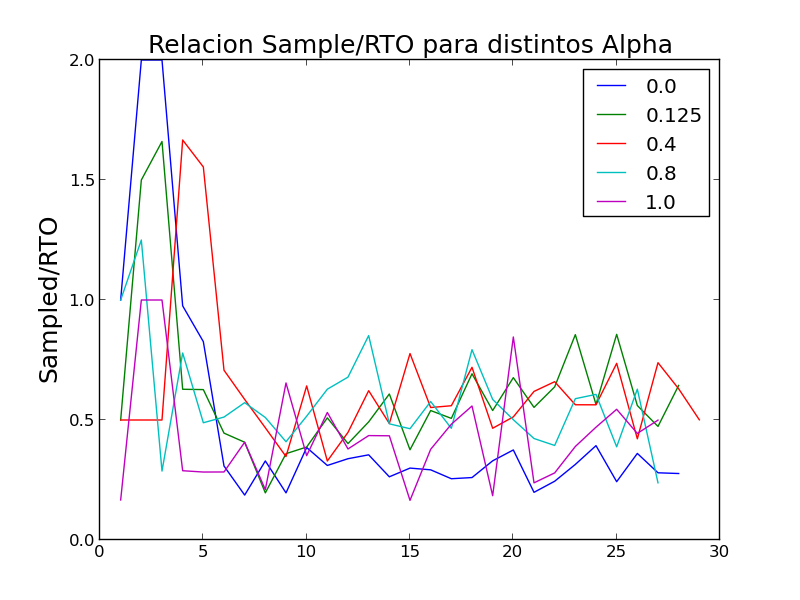
\includegraphics[width=\linewidth]{../graficos/alphavar0drop0.png}
\caption{Relación Sample/RTO, $\beta$ = 0.25}\label{fig:alpha-var0-drop0}
\end{minipage}
\hfill
\begin{minipage}{0.5\linewidth}
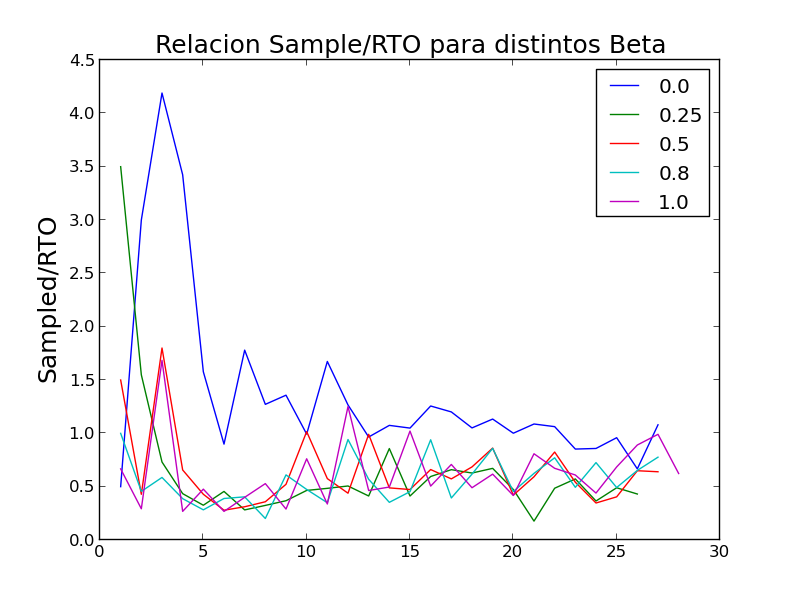
\includegraphics[width=\linewidth]{../graficos/betavar0drop0.png}
\caption{Relación Sample/RTO, $\alpha$ = 0.125}\label{fig:beta-var0-drop0}
\end{minipage}
\end{figure}

\subsubsection{Varianza media}

\begin{figure}[H]
\begin{minipage}{0.5\linewidth}
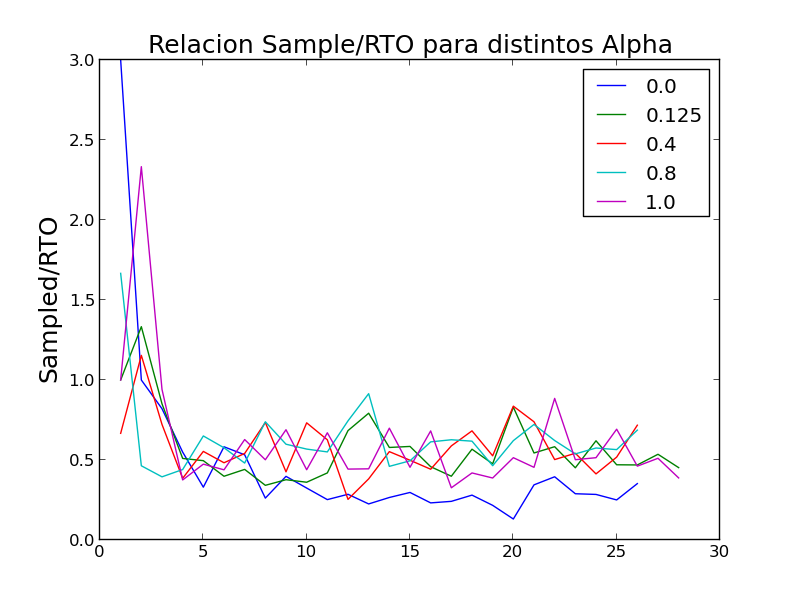
\includegraphics[width=\linewidth]{../graficos/alphavar2drop0.png}
\caption{Relación Sample/RTO, $\beta$ = 0.25}\label{fig:alpha-var2-drop0}
\end{minipage}
\hfill
\begin{minipage}{0.5\linewidth}
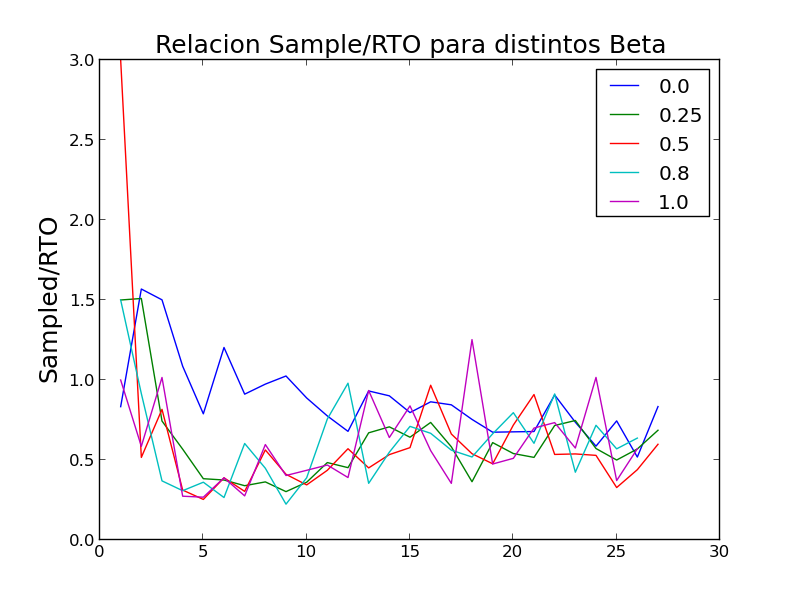
\includegraphics[width=\linewidth]{../graficos/betavar2drop0.png}
\caption{Relación Sample/RTO, $\alpha$ = 0.125}\label{fig:beta-var2-drop0}
\end{minipage}
\end{figure}

\subsubsection{Varianza alta}

\begin{figure}[H]
\begin{minipage}{0.5\linewidth}
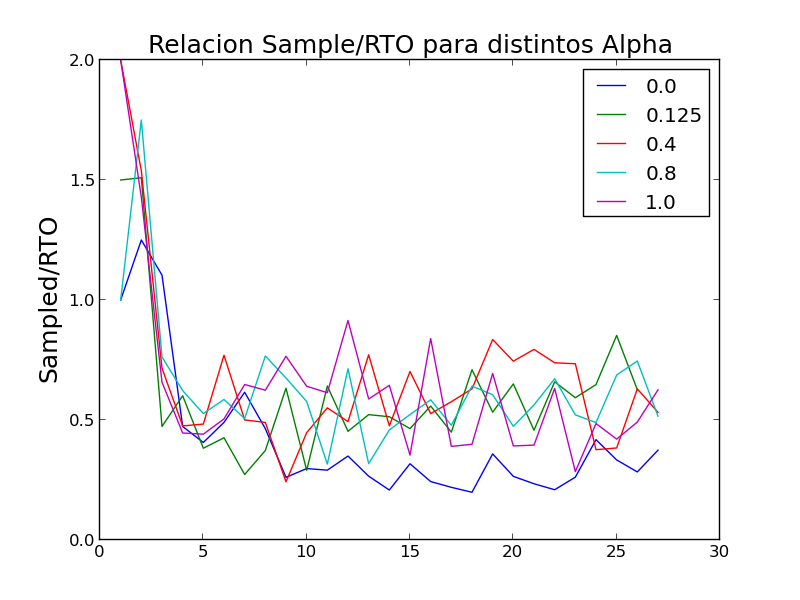
\includegraphics[width=\linewidth]{../graficos/alphavar5drop0.png}
\caption{Relación Sample/RTO, $\beta$ = 0.25}\label{fig:alpha-var5-drop0}
\end{minipage}
\hfill
\begin{minipage}{0.5\linewidth}
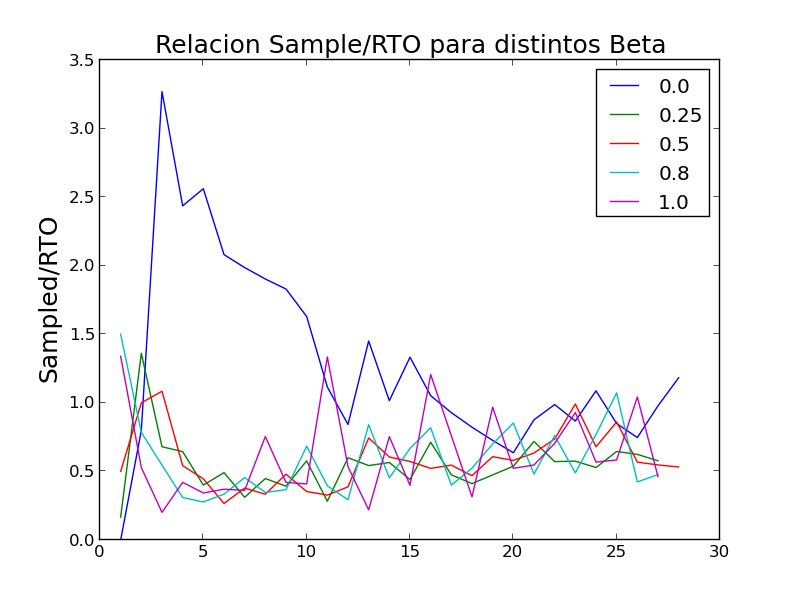
\includegraphics[width=\linewidth]{../graficos/betavar5drop0.png}
\caption{Relación Sample/RTO, $\alpha$ = 0.125}\label{fig:beta-var5-drop0}
\end{minipage}
\end{figure}


\subsection{Drop bajo}
\subsubsection{Sin varianza}

\begin{figure}[H]
\begin{minipage}{0.5\linewidth}
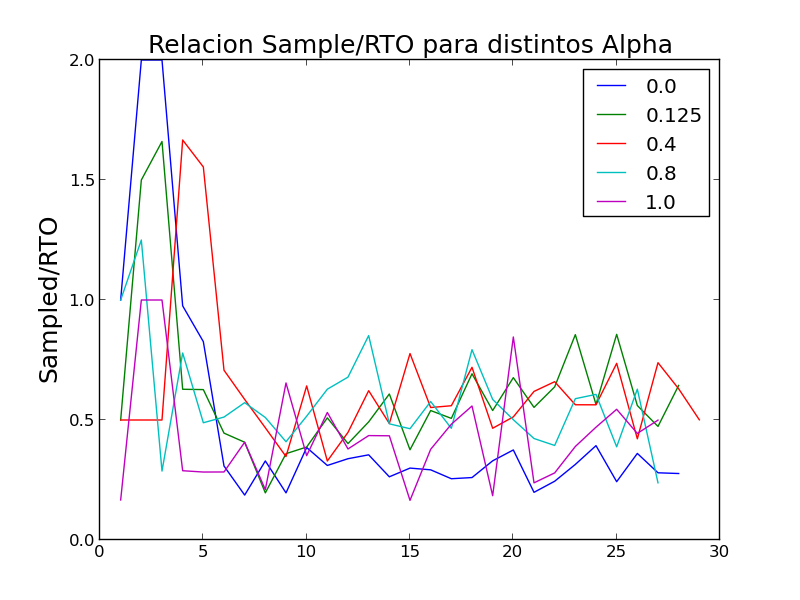
\includegraphics[width=\linewidth]{../graficos/alphavar0drop30.png}
\caption{Relación Sample/RTO, $\beta$ = 0.25}\label{fig:alpha-var0-drop30}
\end{minipage}
\hfill
\begin{minipage}{0.5\linewidth}
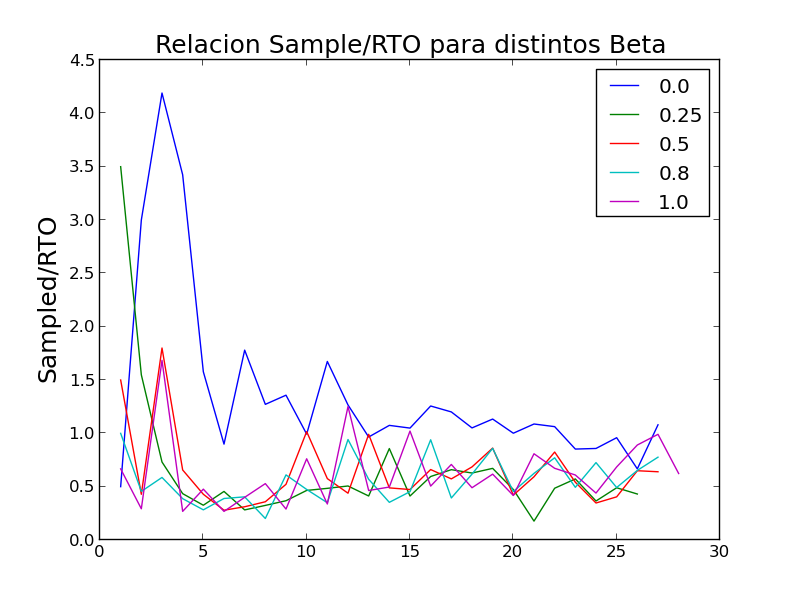
\includegraphics[width=\linewidth]{../graficos/betavar0drop30.png}
\caption{Relación Sample/RTO, $\alpha$ = 0.125}\label{fig:beta-var0-drop30}
\end{minipage}
\end{figure}

\subsubsection{Varianza media}

\begin{figure}[H]
\begin{minipage}{0.5\linewidth}
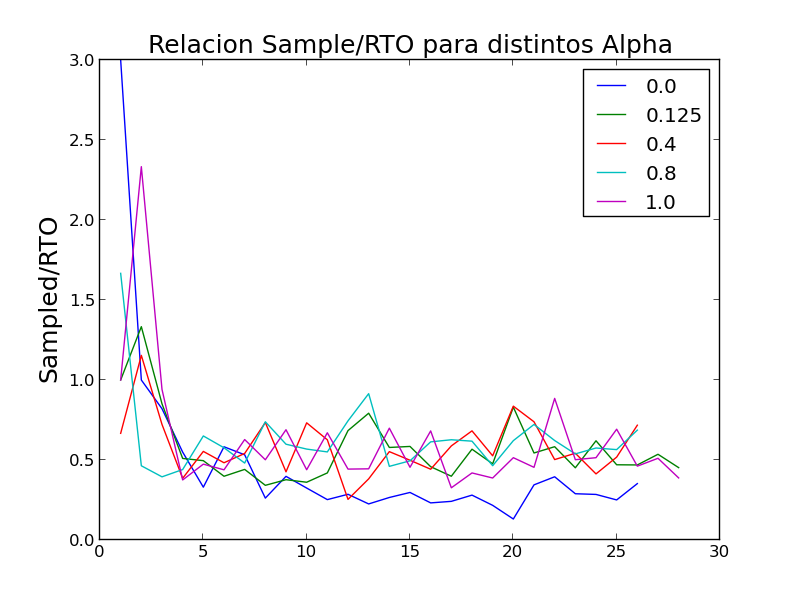
\includegraphics[width=\linewidth]{../graficos/alphavar2drop30.png}
\caption{Relación Sample/RTO, $\beta$ = 0.25}\label{fig:alpha-var2-drop30}
\end{minipage}
\hfill
\begin{minipage}{0.5\linewidth}
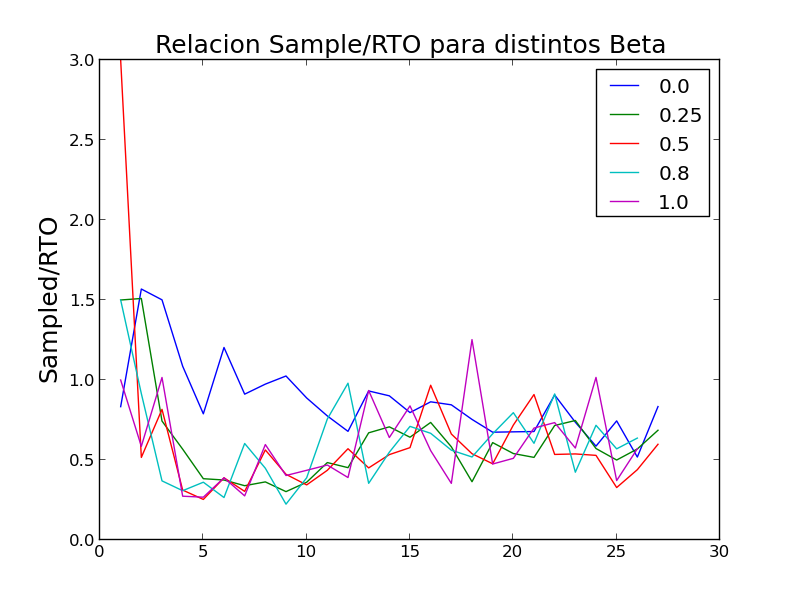
\includegraphics[width=\linewidth]{../graficos/betavar2drop30.png}
\caption{Relación Sample/RTO, $\alpha$ = 0.125}\label{fig:beta-var2-drop30}
\end{minipage}
\end{figure}

\subsubsection{Varianza alta}

\begin{figure}[H]
\begin{minipage}{0.5\linewidth}
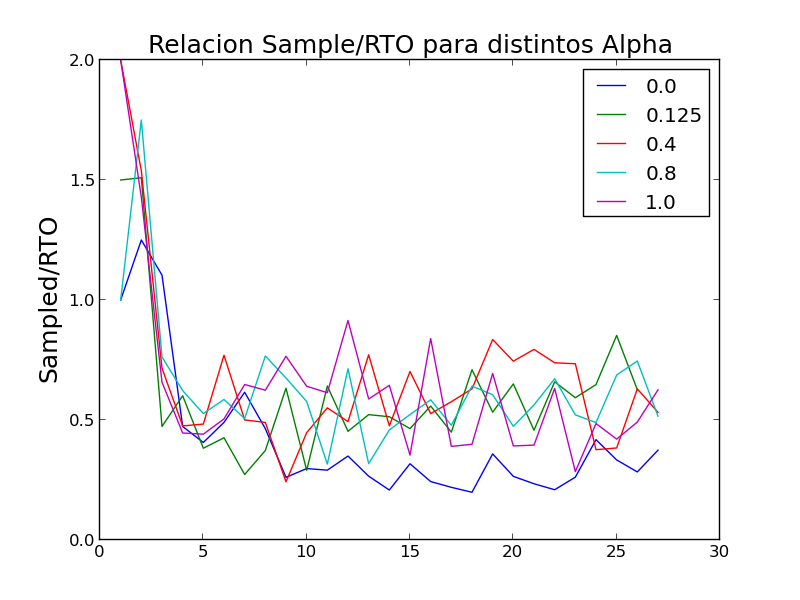
\includegraphics[width=\linewidth]{../graficos/alphavar5drop30.png}
\caption{Relación Sample/RTO, $\beta$ = 0.25}\label{fig:alpha-var5-drop30}
\end{minipage}
\hfill
\begin{minipage}{0.5\linewidth}
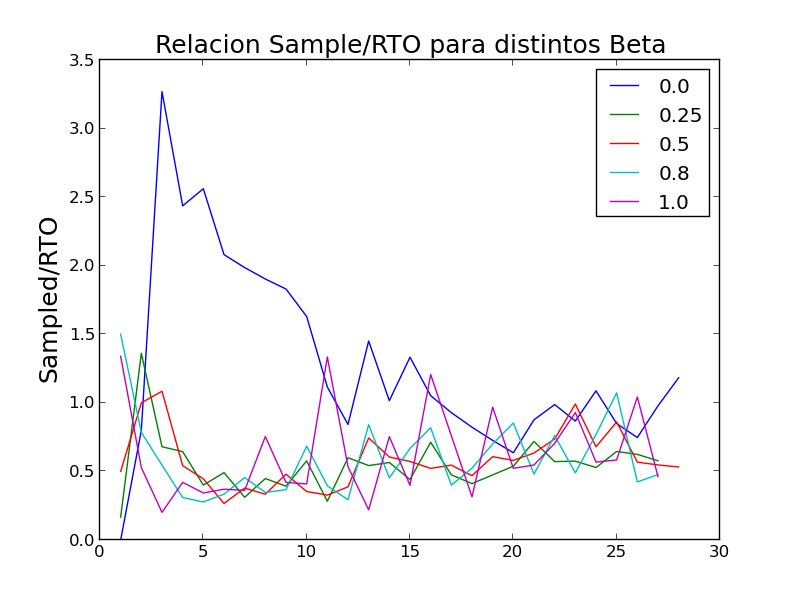
\includegraphics[width=\linewidth]{../graficos/betavar5drop30.png}
\caption{Relación Sample/RTO, $\alpha$ = 0.125}\label{fig:beta-var5-drop30}
\end{minipage}
\end{figure}

\subsection{Drop alto}
\subsubsection{Sin varianza}

\begin{figure}[H]
\begin{minipage}{0.5\linewidth}
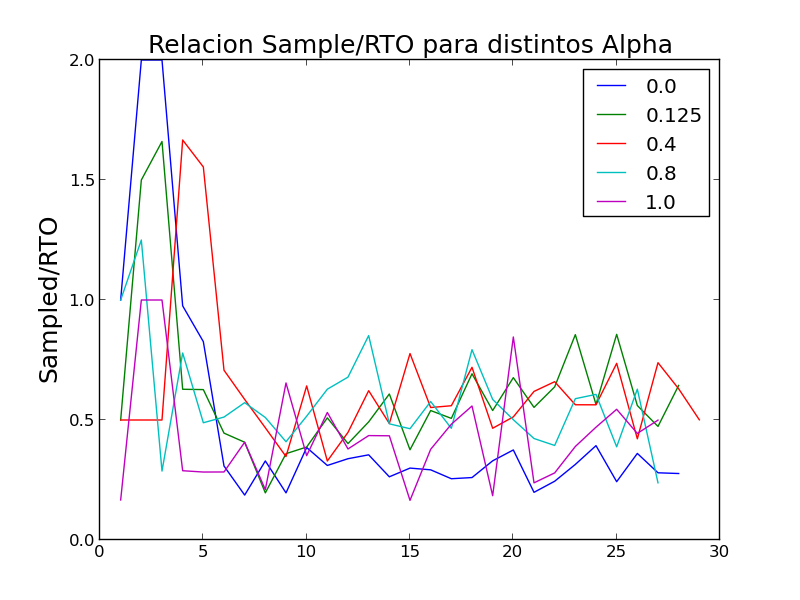
\includegraphics[width=\linewidth]{../graficos/alphavar0drop70.png}
\caption{Relación Sample/RTO, $\beta$ = 0.25}\label{fig:alpha-var0-drop70}
\end{minipage}
\hfill
\begin{minipage}{0.5\linewidth}
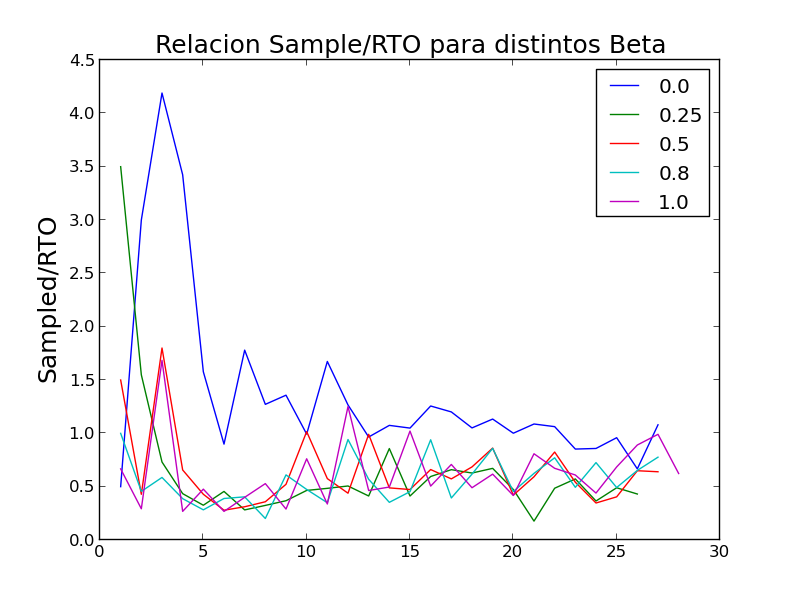
\includegraphics[width=\linewidth]{../graficos/betavar0drop70.png}
\caption{Relación Sample/RTO, $\alpha$ = 0.125}\label{fig:beta-var0-drop70}
\end{minipage}
\end{figure}

\subsubsection{Varianza media}

\begin{figure}[H]
\begin{minipage}{0.5\linewidth}
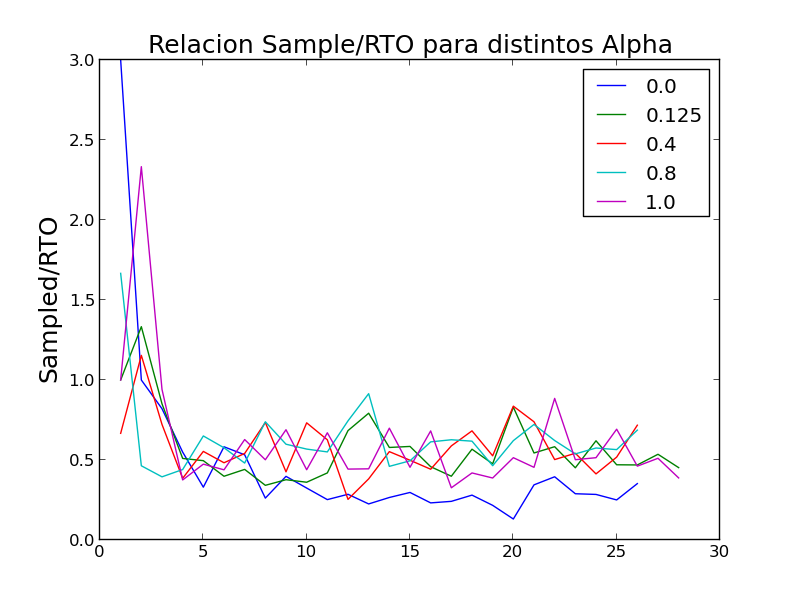
\includegraphics[width=\linewidth]{../graficos/alphavar2drop70.png}
\caption{Relación Sample/RTO, $\beta$ = 0.25}\label{fig:alpha-var2-drop70}
\end{minipage}
\hfill
\begin{minipage}{0.5\linewidth}
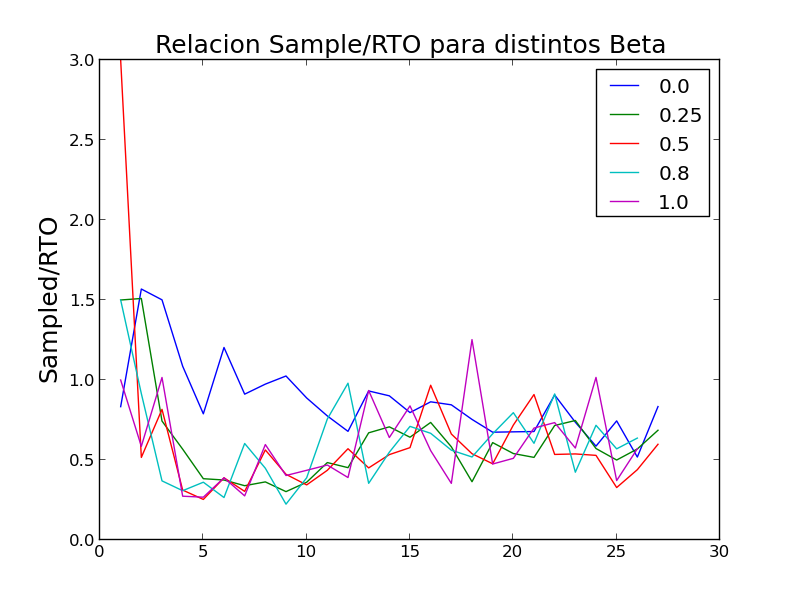
\includegraphics[width=\linewidth]{../graficos/betavar2drop70.png}
\caption{Relación Sample/RTO, $\alpha$ = 0.125}\label{fig:beta-var2-drop70}
\end{minipage}
\end{figure}

\subsubsection{Varianza alta}

\begin{figure}[H]
\begin{minipage}{0.5\linewidth}
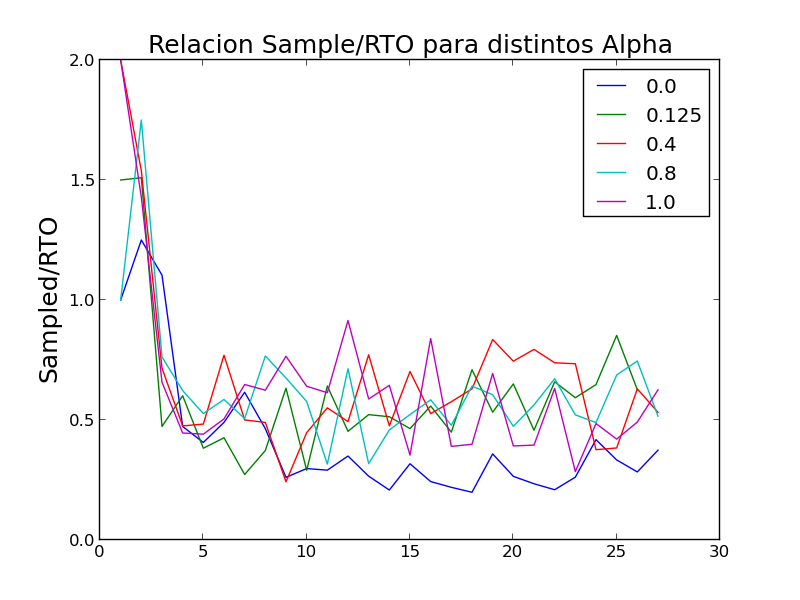
\includegraphics[width=\linewidth]{../graficos/alphavar5drop70.png}
\caption{Relación Sample/RTO, $\beta$ = 0.25}\label{fig:alpha-var5-drop70}
\end{minipage}
\hfill
\begin{minipage}{0.5\linewidth}
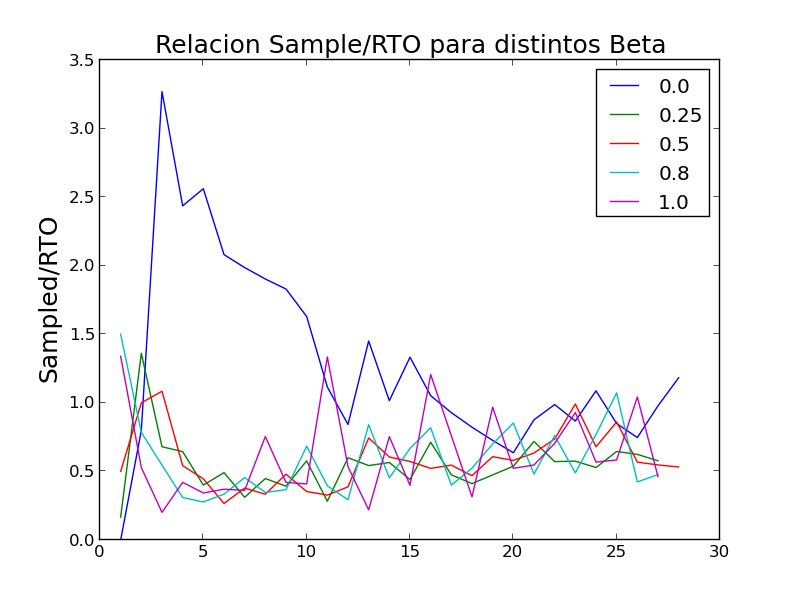
\includegraphics[width=\linewidth]{../graficos/betavar5drop70.png}
\caption{Relación Sample/RTO, $\alpha$ = 0.125}\label{fig:beta-var5-drop70}
\end{minipage}
\end{figure}
\newpage

%%%%%%%%%%%%%%%%%%%%%%%%%%%%%%%%%%%%%%%%%%%%%%%%%%%%%%%%%%%%%%%%%%%%%%%%%%%%%%%
%% Discusión                      	                                      %%
%%%%%%%%%%%%%%%%%%%%%%%%%%%%%%%%%%%%%%%%%%%%%%%%%%%%%%%%%%%%%%%%%%%%%%%%%%%%%%%

\section{Discusión}
\label{sec:discusion}
%TODO falta terminar, te lo pusheo para que veas que fuimos haciendo

En esta sección vamos a discutir acerca de los resultados expuestos en la sección de Resultados.

Observamos que en los gráficos donde la probabilidad de pérdida de paquetes es 0, la cantidad de re-transmisiones es similar para distintas corridas. Esto se debe a que al no haber \emph{dropeos}, se re-envía solamente por \emph{timeout}.

Análogamente, cuando \emph{delay} y la varianza son altos, la cantidad de re-transmisiones en las distintas corridas no son similares sino que hay mucha variabilidad.

Con respecto a $\alpha$, observamos que cuando es 0 la aproximación del \emph{Sampled RTT} respecto al RTO suele ser considerablemente peor respecto del resto de las corridas. Esto lo evidenciamos, por ejemplo, en la Figura \ref{fig:alpha-var0-drop0}.

Esto no se cumple, por ejemplo, cuando tenemos varianza, delay y pérdida de paquetes alto (como podemos ver en la Figura \ref{fig:alpha-var5-drop50-alto}). En estos casos, la relación del \emph{Sampled RTT} respecto del RTO no es buena para ningún $\alpha$. Estos casos los relacionamos con redes reales no estables.
\newpage

%%%%%%%%%%%%%%%%%%%%%%%%%%%%%%%%%%%%%%%%%%%%%%%%%%%%%%%%%%%%%%%%%%%%%%%%%%%%%%%
%% Conclusión                                                                %%
%%%%%%%%%%%%%%%%%%%%%%%%%%%%%%%%%%%%%%%%%%%%%%%%%%%%%%%%%%%%%%%%%%%%%%%%%%%%%%%

\section{Conclusiones}
\label{sec:conclusiones}
Para concluir, nos parece importante recalcar que ningun par de valores de $\alpha$ y $\beta$ es estrictamente mejor que todas las demás. Sin embargo, podemos asegurar que usando valores de $\alpha$ cercanos a 0,125 y $\beta$ cercanos a 0,25 obtuvimos un RTO cercano al \emph{sampled RTT}. Esto confirma que los valores elegidos en el algoritmo de Karn son lo suficientemente buenos.

Otro punto que concluimos es que estos valores de $\alpha$ y $\beta$ siguen estimando el RTT lo suficientemente bien, aún cuando en la red hay delay y/o pérdida de paquetes altas.

Para finalizar, queremos 

\end{document}